\pagestyle{fancy}
\fancyhead{} % clear all header fields
\fancyhead[LO,CE]{Réalisation}
\fancyhead[RO,LE]{2024-2025}

\chapter{Réalisation du projet}
\section{Mise en place de l'environnement de développement}
\subsection{Configuration de Firebase Realtime Database}
Dans Firebase, tout est organisé dans des projets afin de pouvoir regrouper les ressources et de facilité la gestion des règles et poliques de sécurité. La première étape est donc de créer un projet dans Firebase, illustré sur la figure~\ref{fig:creation_projet_dans_firebase}.


\begin{figure}[H]
   \centering
   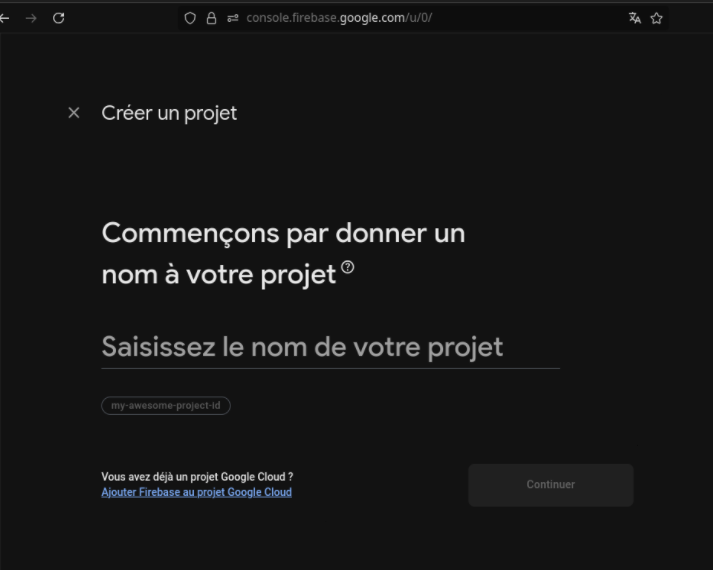
\includegraphics[scale=0.5]{firebase-project-setup.png}
   \caption{Création de projet dans Firebase}
   \label{fig:creation_projet_dans_firebase}
\end{figure}

Ensuite, on doit activer Firebase Authentication afin de pouvoir l'utiliser comme méthode d'authentification dans l'application mobile. Dans le console d'administration de Firebase, il faut passer sur \textbf{Créer > Authentication > Méthode de connexion > Ajouter un fournisseur > Adresse e-mail/Mot de pase}, puis d'activer la fonctionnalité comme illustré dans la figure~\ref{fig:activation_de_Firebase_Auth}.

\begin{figure}[H]
   \centering
   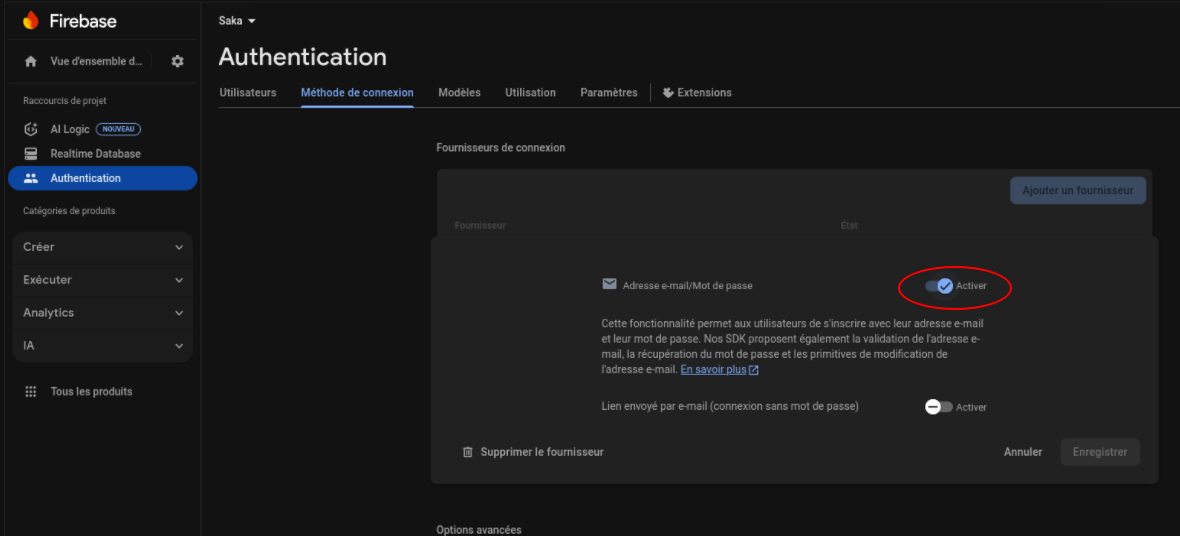
\includegraphics[scale=0.5]{firebase_auth.png}
   \caption{Activation de Firebase Authentication}
   \label{fig:activation_de_Firebase_Auth}
\end{figure}

Pour créer l'instance de Realtime Database, il faut passer par \textbf{Créer > Realtime Database > Créer une base de données}, puis suivre les étapes de reglage des options et des règles de sécurité. Une fois activé, on obtient un lien illustré sur la  figure~\ref{fig:db_dans_realtime_db}.

\begin{figure}[H]
   \centering
   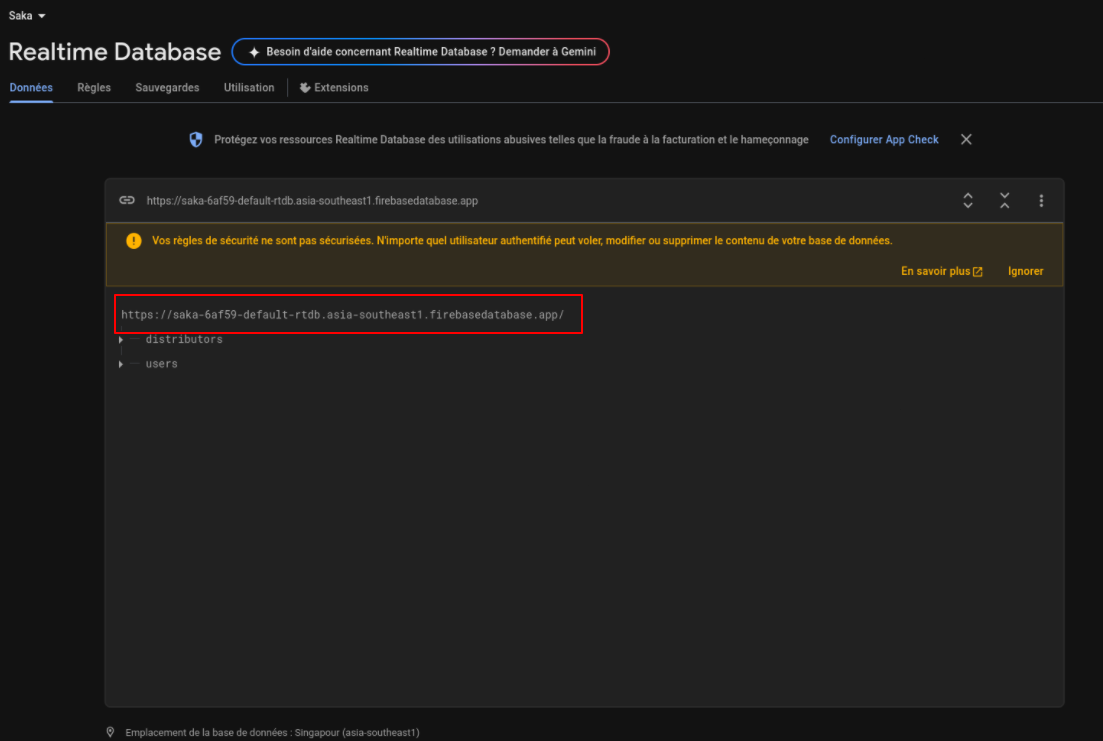
\includegraphics[scale=0.6]{firebase_realtime_db.png}
   \caption{La base de données dans Realtime Database}
   \label{fig:db_dans_realtime_db}
\end{figure}

\section{Développement de l'application mobile}
\section{Développement du serveur websocket}
\section{Montage du système et réglages matériels}
